Aligning DNA is a complex task because of how large the sample and the reference can be. In the case of the human genome, the complete genome size is around 3.4GB when stored in plain text, meaning, having the full sequence of letters A, T, C and G to represent the DNA. While this could seem fairly unimpressive (after all, it could fit on a regular DVD without any kind of compression), looking for a particular area that would match is far from trivial. As such, a sophisticated way to look into the genome and find an alignment is needed.

Aligning DNA is a computing challenge that asks for various techniques to achieve it in a timely manner. The problem at stake is then to find an effective way to compute DNA alignment as fast as possible.

At the moment, DNA alignments represents the first genomics analysis steps of almost every single DNA analysis approach in practice. In addition, alignment algorithms are rather time consuming, both due to the high complexity of the analysis involved as well as the amount of data that needs to be processed. In many cases, alignment consumes about $50\%$ of the total DNA analysis time. We can see on Figure~\ref{fig:pipelineprocesstime} that the time taken by alignment, also called "mapping", is about a third of the total pipeline time. Moreover, the time taken for this part is counted in thousands of CPU-core hours for this example data set: this shows that speeding it up should result in important savings in runtime.

\begin{figure}[h]
	\centering
	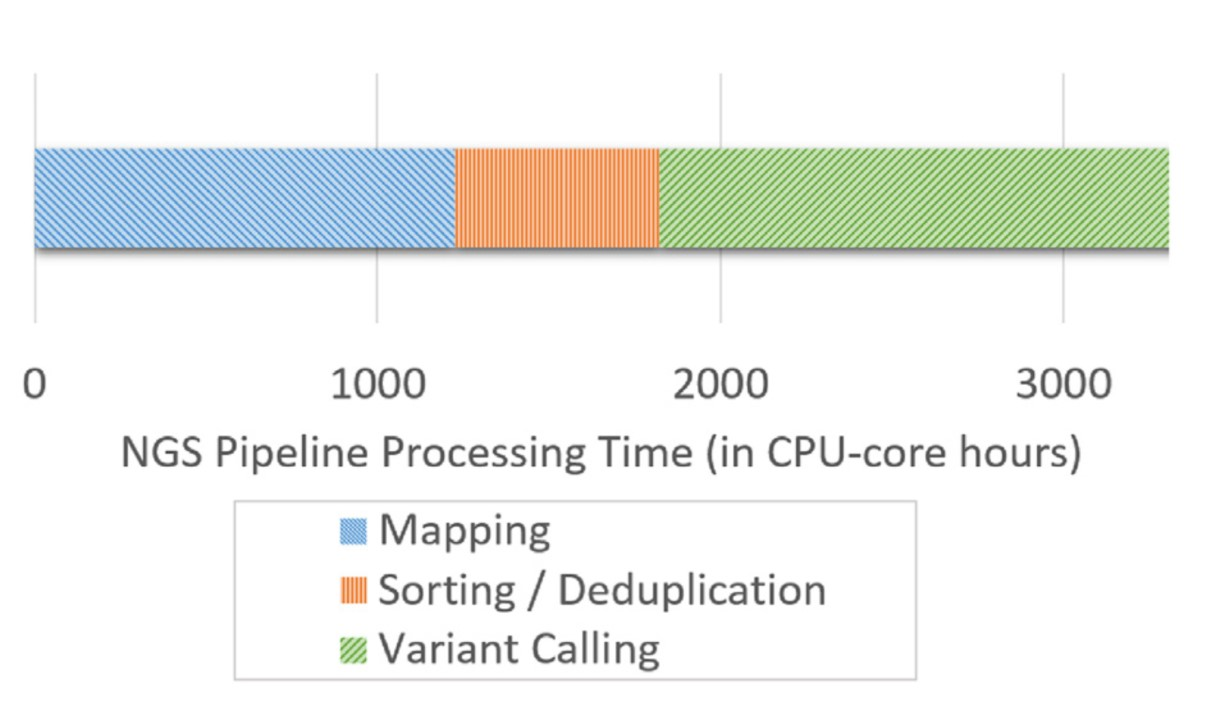
\includegraphics[width=1\linewidth]{pipelineprocesstime}
	\caption{DNA pipeline process time share for a typical 30$\times$ coverage cancer DNA data set. The data set consists of three tumor samples and one normal tissue sample (time given in CPU-core hours). (from~\cite{HOUTGAST201854})}
	\label{fig:pipelineprocesstime}
\end{figure}


% refer to that paper : https://www.sciencedirect.com/science/article/pii/S1476927118301555 and also show the figure in the paper (copy it and use a reference)
